\subsection{Statistics}

\begin{question}
    Why can MLE be used so uniformly?
\end{question}

\textbf{Maximum likelihood estimation} (MLE) and \textbf{maximum a posterior estimation} (MAP):
$\hat{\bm{\theta}}_{MLE}$ -- the parameters' estimation that assign the highest probability to the observations;
$\hat{\bm{\theta}_{MAP}}$ -- the parameters' estimation maximizing the posterior probability under some priori $\pi(\bm{\theta})$. 
If \uline{the priori is a uniform distribution}, 
then $\hat{\bm{\theta}}_{MLE}=\hat{\bm{\theta}}_{MAP}$.\unsure{
Reason 1
}
\begin{gather}
    \hat{\bm{\theta}}_{MLE}
    \triangleq \argmax_{\bm{\theta}}p(\mathcal{D}|\bm{\theta})\\
    \hat{\bm{\theta}}_{MAP}
    \triangleq \argmax_{\bm{\theta}}p(\bm{\theta}|\mathcal{D})
    = \argmax_{\bm{\theta}}p(\mathcal{D}|\bm{\theta})\pi(\bm{\theta})
\end{gather}
\textbf{Kullback Leibler divergence} (KL divergence): 
A standard way to measure the dissimilarity between probability distribution $p$ and $q$.
\begin{align}
    \infdiv{p}{q}
    =& \sum_{\bm{y}}{p(\bm{y})\log\frac{p(\bm{y})}{q(\bm{y})}}\\
    =& \underbrace{\sum_{\bm{y}}{p(\bm{y})\log p(\bm{y})}}_{-\mathbb{H}(p)\text{:entropy}}
    - \underbrace{\sum_{\bm{y}}{p(\bm{y})\log q(\bm{y})}}_{-\mathbb{H}_{\text{CE}}(p,q)\text{:cross-entropy}}
\end{align}
If \uline{$q(\bm{y})=p(\bm{y}|\bm{\theta})$ and $p(\bm{y})=p_\mathcal{D}(\bm{y})$}, 
then $\infdiv{p}{q}=\text{const}+\mathrm{NNL}(\bm{\theta})$.\unsure{Reason 2}
which shows the relationship between MLE and KL divergence.
And above all justify usage of MLE from the perspectives of Bayesain and empirical distribution.

\begin{example}
    \textbf{MLE for linear regression} aka\\
    \textbf{ordinary least squares} or OLS estimate
    \begin{align}
        p(y|\bm{x};\bm{\theta})
        =& \mathcal{N}(\bm{w}^T\bm{x},\sigma^2)\\
        \hat{\bm{w}}_{OLS}\equiv\hat{\bm{w}}_{MLE}
        \triangleq& \argmin_{\bm{w}}\text{NLL or RSS or MSE or RMSE}\\
        =& (\bm{X}^T\bm{X})^{-1}\bm{X}^T\bm{y}
    \end{align}
\end{example}

\textbf{Empirical risk minimization} (ERM) 
\begin{gather}
    \mathcal{L}(\bm{\theta})=\frac{1}{N}\sum_{n=1}^N\ell(\bm{y}_n,\bm{\theta};\bm{x}_n)
\end{gather}
where $\ell(\cdot)$ is any loss function that measures the mismatchness with expected outcomes, 
(if $\ell(\bm{y}_n,\bm{\theta};\bm{x}_n)=-\log{p(\bm{y}_n|\bm{\theta},\bm{x}_n)}$,
then $\mathcal{L}(\bm{\theta})=\text{NLL}(\bm{\theta})$ and ERM is MLE).\unsure{Reason 3}
% \textbf{Surrogate loss function}: 
% The surrogate is usually chosen to be a maximally tight
% convex upper bound, which is then easy to minimize, e.g. 

% \begin{enumerate}[(i)]
%     \item 0-1 loss: 
%     $\ell_{01}(\bm{y}_n,\bm{\theta};\bm{x}_n)=\mathbb{I}(\bm{y}_n\neq f(\bm{x}_n;\bm{\theta})$
%     \item :
    
% \end{enumerate}

\begin{figure}[hptb]
    \centering
    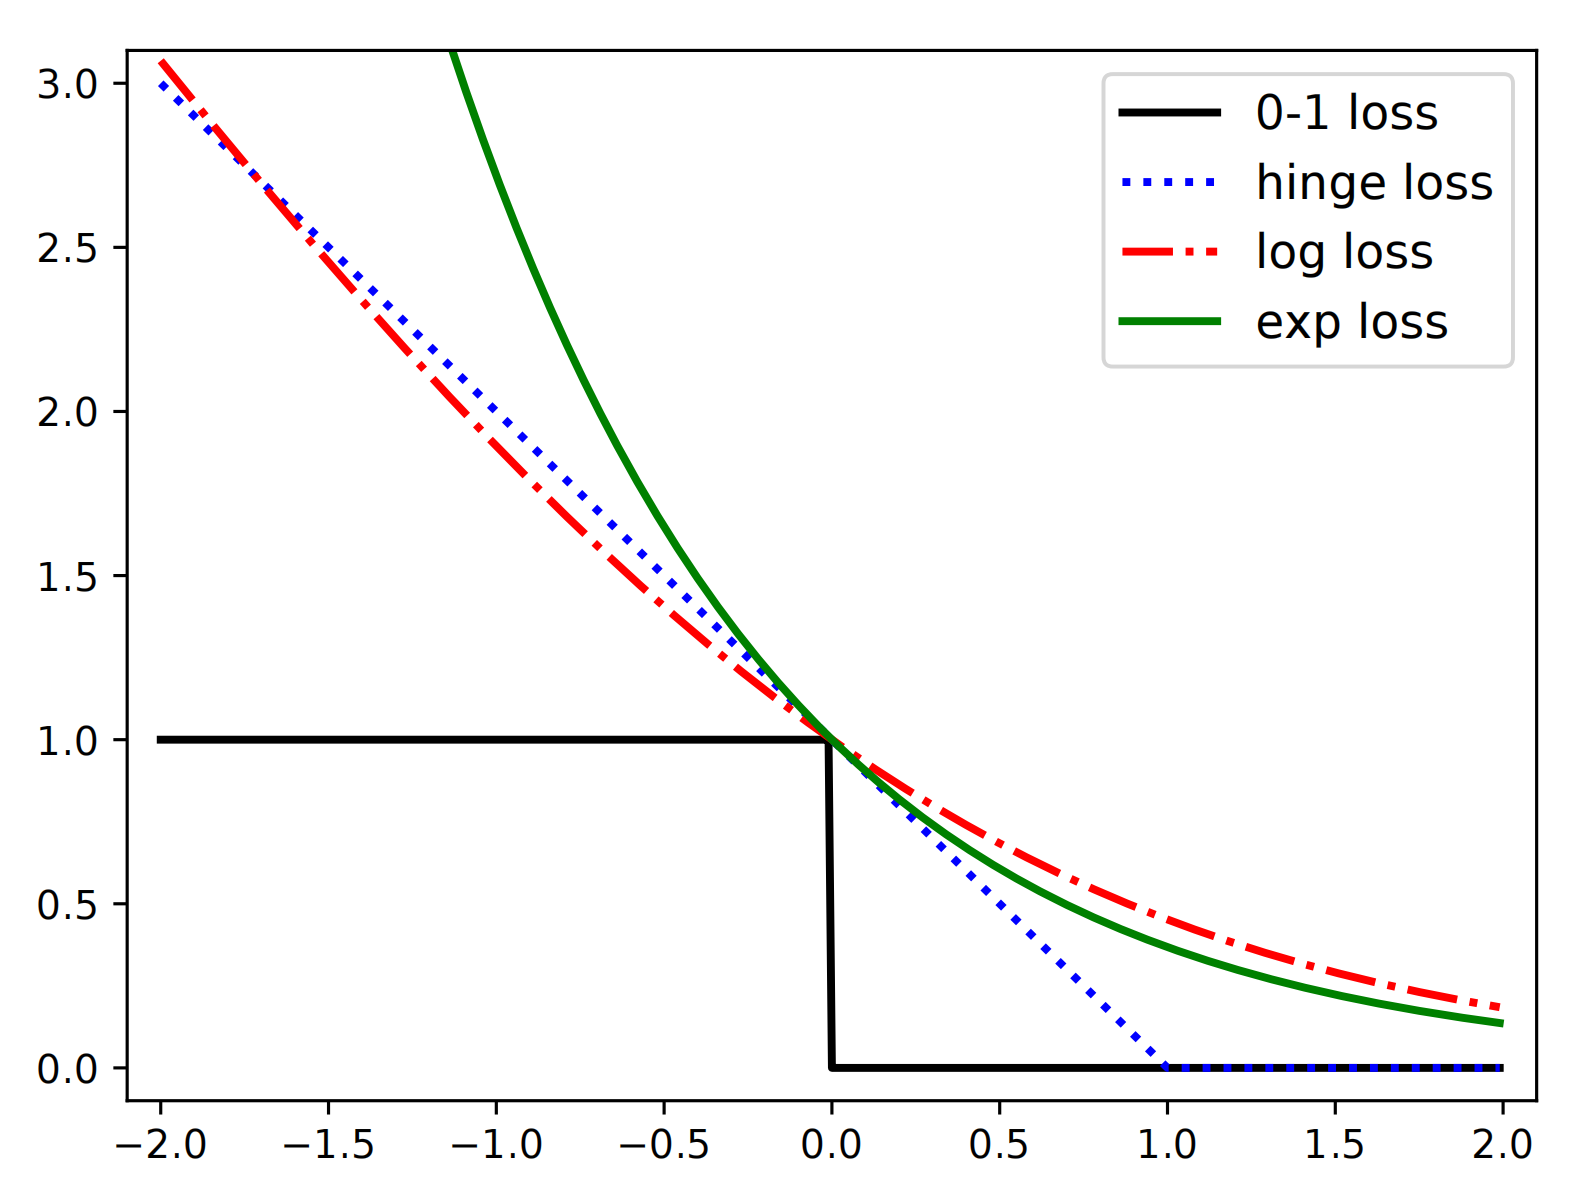
\includegraphics[width=0.5\textwidth]{figs/lossfunc.png}
    \caption{Loss functions for \uline{binary classifiers}}
    {\footnotesize Horizontal axis: $z=yf(\bm{x};\bm{\theta})$. \\
    0-1 loss: $\mathbb{I}(z<0)$;
    Hinge loss: $\max\{0,1-z\}$;
    Log-loss: $\log_2{(1+e^{-z})}$;
    Exp-loss: $e^{-z}$.}
    \label{fig:lossfunc}
\end{figure}

\textbf{Estimation method of moments} (MOM): 
equate the \uline{theoretical moments (functions of parameters)},
to the \uline{empirical moments},
where we need the same number of simultaneous equations for solving $K$ unknown parameters,
to avoid difficult computation in MLE 
but with less efficiency of data usage, so can be used to initialize iterative algorithms for MLE.

\textbf{Online (recursive) estimation} with recursive update $f$:
\begin{gather}
    \hat{\bm{\theta}}_t=f(\hat{\bm{\theta}}_{t-1},\bm{y}_t)
\end{gather}

\begin{example}
    \textbf{Exponentially-weighted moving average} (EWMA)
    \begin{align}
        \hat{\bm{\mu}}_t
        =& \beta\hat{\bm{\mu}}_{t-1}+(1-\beta)\hat{\bm{y}}_t\\
        =& \beta^t\bm{y}_0 + (1-\beta)\beta^{t-1}\bm{y}_1 + \cdots + (1-\beta)\beta\bm{y}_{t-1} + (1-\beta)\bm{y}_t
    \end{align}
    where a smaller $\beta$ forgets the past data more quickly and 
    adapts to the more recent data more rapidly.
\end{example}

\textbf{Regularization} term $C(\bm{\theta})$ in the loss function is 
a given measure for the parameters' complexity to avoid overfitting:
\begin{gather}
    \mathcal{L}(\bm{\theta};\lambda)
    = \frac{1}{N}\sum_{n=1}^N\ell(\bm{y}_n,\bm{\theta};\bm{x}_n)
    + \lambda C(\bm{\theta})
\end{gather}
where $C(\bm{\theta})$ can be some $-\log{\pi(\bm{\theta})}$,
then objective become a MAP estimation for a given priori $\pi(\bm{\theta})$ for $\lambda=1$.
e.g. add-one smoothing (or \textbf{Laplace's rule of succession}) in Bernoulli distribution with $\pi\sim\text{Beta}(2,2)$ $p\sim$ and shrinkage estimation for $\Sigma$ in multivariate Gaussian with $\pi\sim$ inverse Wishart. 

\textbf{Bayes model averaging} (BMA): make predictions under the posterior distribution of parameters, which weighted the predictions for all possible parameters (models)
\begin{gather}
    \pi(\bm{\theta}|\mathcal{D})
    = \frac{\pi(\bm{\theta})p(\mathcal{D}|\bm{\theta})}{p(\mathcal{D})}\\
    p(\bm{y}|\bm{x},\mathcal{D})
    = \int{p(\bm{y}|\bm{x};\bm{\theta})\pi(\bm{\theta}|\mathcal{D})}d\bm{\theta}
\end{gather}
where $\bm{x}$ is new observations, $\mathcal{D}$ is training data, and 
$p(\bm{y}|\bm{x},\mathcal{D})$ is the final averaging model.


\textbf{Mixtures of priors} by introducing a latent indicator variable $h$
\begin{gather}
    \pi(\bm{\theta})=\sum_k p(h=k)\pi(\bm{\theta}|h=k)
\end{gather}
$\Rightarrow$
\begin{align}
    \pi(\bm{\theta}|\mathcal{D})
    =& \sum_k{p(h=k|\mathcal{D})p(\bm{\theta}|\mathcal{D},h=k)}\\
    p(h=k|\mathcal{D})
    =& \frac{p(h=k)p(\mathcal{D}|h=k)}{\sum_{k'}{p(h=k')p(\mathcal{D}|h=k')}}
\end{align}
\improvement{
The detailed discussion on 
prior, posterior, predictive, and marginal likelihood of
(1) Beta-Binomial, (2)\textbf{Dirichlet-Multinomial}, and (3) Gaussian-Gaussian
are skipped.
}

\textbf{Other priors} besides conjugate priors
\begin{enumerate}[(1)]\label{kspt:noninfo}
    \item \textbf{noninformative prior} or preferred \textbf{minimally informative prior}: 
    let the data speak for itself, 
    e.g. \textbf{flat prior} $\pi\propto 1$ in Gaussian;
    \item \textbf{hierarchical prior}: the hyperparameters in prior also follow some prior --
    $\bm{\phi}\to\bm{\theta}\to\mathcal{D}$;
    \item \textbf{empirical prior}: the prior's hyperparameters $\bm{\phi}$ directly estimated from data $\mathcal{D}$ as shown below
    \begin{gather}
        \hat{\bm{\phi}}(\mathcal{D})
        = \argmax_{\bm{\phi}}p(\mathcal{D}|\bm{\phi})
        = \argmax_{\bm{\phi}}\int{p(\mathcal{D}|\bm{\theta})p(\bm{\theta}|\bm{\phi})}d\bm{\theta}
    \end{gather}
    which is called \textbf{Empirical Bayes} (EB).
\end{enumerate}

Available inference methods:
\begin{itemize}
    \item MLE:
    \begin{gather}
        \hat{\bm{\theta}}
    =\argmax_{\bm{\theta}}
    p(\mathcal{D}|\bm{\theta})
    \end{gather}
    \item MAP: 
    \begin{gather}
        \hat{\bm{\theta}}
    =\argmax_{\bm{\theta}}
    p(\mathcal{D}|\bm{\theta})p(\bm{\theta}|\bm{\phi})
    \end{gather}
    \item MLE-II (EB):
    \begin{gather}
        \hat{\bm{\phi}}
    =\argmax_{\bm{\phi}}
    \int{p(\mathcal{D}|\bm{\theta})p(\bm{\theta}|\bm{\phi})}d\bm{\theta}
    \end{gather}
    \item MAP-II:
    \begin{gather}
        \hat{\bm{\phi}}
    =\argmax_{\bm{\phi}}
    \int{p(\mathcal{D}|\bm{\theta})p(\bm{\theta}|\bm{\phi})p(\bm{\phi})}d\bm{\theta}
    \end{gather}
    \item Full Bayes:
    \begin{gather}
        p(\bm{\theta},\bm{\phi}|\mathcal{D})
    \propto p(\mathcal{D}|\bm{\theta})p(\bm{\theta}|\bm{\phi})p(\bm{\phi})
    \end{gather}
\end{itemize}

\textbf{Computational issues} in Bayesian ML: 
It is usually \uline{intractable to compute $p(\bm{\theta}|\mathcal{D})$}
given $p(\mathcal{D}|\bm{\theta})$ and $p(\bm{\theta})$.
Therefore, methods of \textbf{approximate posterior inference} are necessary.
\begin{itemize}
    \item \textbf{Grid approximation}:  
    brute-force enumerate finite set in partition the space of possible values $\bm{\theta}$.
    \begin{gather}
        p(\bm{\theta}=\bm{\theta}_k|\mathcal{D})
        \approx \frac{p(\mathcal{D}|\bm{\theta}_k)}{\sum_{k'=1}^K{p(\mathcal{D},\bm{\theta}_{k'})}}
    \end{gather}
    \item \textbf{Quadratic (Laplace) approximation}: 
    approximate the posterior by a multivariable Gaussian.
    $\mathcal{E}(\bm{\theta})=-\log{p(\bm{\theta},\mathcal{D})}$ is an \textbf{energy function}, 
    $\hat{\bm{\theta}}$ is the mode ($\Rightarrow\nabla{\mathcal{E}(\bm{\theta})}|_{\bm{\theta}=\hat{\bm{\theta}}}=\bm{0}$), 
    at which $\mathbf{H}$ is Hessian of $\mathcal{E}$.
    \begin{gather}
        p(\bm{\theta}|\mathcal{D})
        \approx \mathcal{N}(\hat{\bm{\theta}},\mathbf{H}^{-1})
    \end{gather}
    \item \textbf{Variational approximation}: 
    find a $q$ minimizing \uline{some discrepancy $D$}, say KL divergence, with target posterior
    in tractable family of distribution $\mathcal{Q}$,
    \begin{gather}
        p(\bm{\theta}|\mathcal{D})
        \approx q^*=\argmin_{q\in\mathcal{Q}} \infdiv{q}{p}
    \end{gather}
    \item \textbf{Monte Carlo approximation}: 
    build an empirical distribution of $\bm{\theta}$ by
    \uline{efficiently create a postrior sample of parameters} $\{\Tilde{\bm{\theta}}_s\}_{s=1}^S\sim p(\bm{\theta}|\mathcal{D})$, 
    without having to evaluate the normalization constant $p(\mathcal{D})$, then
    \begin{gather}
        p(\bm{\theta}|\mathcal{D})
        \approx\frac{1}{S}\sum_{s=1}^S\delta(\bm{\theta}-\Tilde{\bm{\theta}}_s)
    \end{gather}
\end{itemize}

\textbf{Uncertainty represented by \textit{frequentist}}:
$\hat{\bm{\theta}}=\pi(\mathcal{D})$ the estimator's distribution,
\textbf{sampling distribution},
depends on the random data and it is also a r.v..\unsure{
This idea is the same with what we have learnt in STAT5010 for all estimator, 
function of observations, of some transformation of true parameter $g(\bm{\theta})$.
}
However, in the view of frequentist, 
there exists a true single value $\bm{\theta}^*$ that generates the data $\mathcal{D}\sim p(\bm{x}|\bm{\theta}^*)$.
We can find the distribution of $\hat{\bm{\theta}}$, 
$p(\pi(\mathcal{D})=\bm{\theta}|\mathcal{D}\sim\bm{\theta}^*)$ analytically if it is tractable.
If the transformation is intractable, computational issues occur, like in Bayes ML above, and 
then approximation methods are also needed.
\begin{itemize}
    \item \textbf{Gaussian approximation}: \info{
    Gaussian approximation is applied in C-SIDE to model the uncertainty of $\hat{\bm{\beta}}$ for testing $H_0:\bm{\beta}^*=0$}
    by the asymptotic normality of CLT (Theorem \ref{thm:asymnorm}), the distribution of MLE converges to Gaussain
    \begin{gather}
        p(\pi(\mathcal{D})=\bm{\theta}|\mathcal{D}\sim\bm{\theta}^*)
        \to
        \mathcal{N}(\bm{\theta}^*,1/N\mathbf{I}(\bm{\theta}^*))
    \end{gather}
    \item \textbf{(Non-parametric) bootstrap approximation}: a kind of MC technique,
    the distribution of $\hat{\bm{\theta}}$ is approximated 
    by the \uline{empirical distribution from observed data}:
    \begin{gather}
        p(\pi(\mathcal{D})=\bm{\theta}|\mathcal{D}\sim\bm{\theta}^*)
        \approx \frac{1}{S}\sum_{s=1}^S\delta(\bm{\theta}-\pi(\Tilde{\mathcal{D}}_s))
    \end{gather}
    The key of bootstrap is to sample $S$ new datasets $\{\Tilde{\mathcal{D}}_s\}$ with the same size with and from the original dataset,
    $\Tilde{\mathcal{D}}$, with replacement.
    $N:=|\Tilde{\mathcal{D}}|=|\Tilde{\mathcal{D}}_s|$,
    the probability an item is picked at least once is 
    $1-\left(1-\frac{1}{N}\right)^N\to1-e^{-1}$.\unsure{
    Relationship sampling distribution and posterior distribution:
    recall the minimally informative prior in $\S$ \ref{kspt:noninfo}. 
    Sampling distribution only relies on the data.
    }
\end{itemize}


\begin{theorem}\label{thm:asymnorm}
    \textbf{Asymptotic normality}\footnote{
    \citep{pml1Book} Thm 4.7.1
    }\\
    If the parameters are identifiable, then
    \begin{gather}
        p(\pi(\mathcal{D})=\bm{\theta}|\mathcal{D}\sim\bm{\theta}^*)
        \to
        \mathcal{N}(\bm{\theta}^*,1/N\mathbf{I}(\bm{\theta}^*))
    \end{gather}
    where $\mathbf{I}(\bm{\theta}^*)$ is the \textbf{Fisher information matrix} defined as
    \begin{gather}
        \mathbf{I}(\bm{\theta})
        \triangleq\mathbb{E}_{\bm{X}|\bm{\theta}}\left[ 
            (\nabla_{\bm{\theta}}\log{p(\bm{X}|\bm{\theta})})
            (\nabla_{\bm{\theta}}\log{p(\bm{X}|\bm{\theta})})^T
        \right]
    \end{gather}
\end{theorem}

\begin{theorem}
    \textbf{Log-likelihood with twice differentiability}\footnote{
    \citep{pml1Book} Thm 4.7.2
    }\\
    If $\log p(\bm{X}|\bm{\theta})$ is twice differentiable, and under certain regularity conditions,
    \begin{gather}
        \mathbf{I}(\bm{\theta})
        =-\mathbb{E}_{\bm{X}|\bm{\theta}}\left[ 
            (\nabla_{\bm{\theta}}^2\log{p(\bm{X}|\bm{\theta})})
        \right]
    \end{gather}
    which is \uline{Hessian of NLL}.
    \uline{A log-likelihood function with high curvature (large Hessian) will result in
    a low variance estimate, since the parameters are ``well determined'' by the data,
    and hence robust to repeated sampling.}
\end{theorem}\unsure{
Good intuitive understanding. This theorem is also introduced in STAT5010.
}



\textbf{Difference between \uline{credible interval} and \uline{confidence interval}}:
Credible interval: $\mathcal{D}$ fixed (since observed), $\theta$ random;
confidence interval: $\mathcal{D}$ random, $\theta^*$ fixed.
Confidence interval $I(\Tilde{\mathcal{D}})$ such that $P(\theta^*\in I(\Tilde{\mathcal{D}})|\Tilde{\mathcal{D}}\sim\theta^*)=0.95$ \textbf{\textit{does not}} mean that
the true parameter $\theta^*$ is 95\% likely to live inside $I(\Tilde{\mathcal{D}})$, 
which, however, is exactly the quantity given by credible interval {\color{red}$P(\theta\in I|\mathcal{D})$???}.
Confidence interval will cover the true parameter $100(1-\alpha)\%$ of the time.\unsure{
very confusing concept that I still do not understand...
}

% \begin{example}
%     \mathcal{D}=(y_1,y_2) from 
%     \begin{gather}
%         p(y|\theta)=\begin{array}{ll}
%             0.5 & \text{if}~y=\theta \\
%             0.5 & \text{if}~y=\theta+1 \\
%             0 & \text{otherwise}
%         \end{array}
%     \end{gather}
%     If $\theta=39$ and we will obtain the each of data, 
%     $\{(39,39),(39,40),(40,39),(40,40)\}$, 
%     with proba. 0.25
    
% \end{example}

% \textbf{Bias-variance trade-off}


% \textbf{Confidence interval}: uncertainty of a parameter estimate.
% It is worth noting that $p(\pi(\mathcal{D})=\bm{\theta}|\mathcal{D}\sim\bm{\theta}^*)$ 
% is not distribution of true $\bm{\theta}^*$ (with not uncertainty)
% but a guess (r.v.) from data with certain change covering the unknown true $\bm{\theta}^*$.
% \textbf{$100(1-\alpha)\%$ confidence interval} is \uline{any} interval\unsure{
% recall credable region
% }

% \subsection{Decision Theory}

% \subsection{Information Theory}

\subsection{Linear Algebra}

% \subsection{Optimization}